\section{Final Velocity Model}
\eqref{eq:Totaltorquewithcurrentexpression} delivers the information needed to make a visual representation of the motor model. The input is the supply voltage, \si{V_m(s)} delivered to the motor and the output is the required torque, \si{\tau_m}, see \figref{fig:motormodelBlock}. The block representation of the system is used, when the system is to be simulated.

\begin{figure}[H]
	\centering
	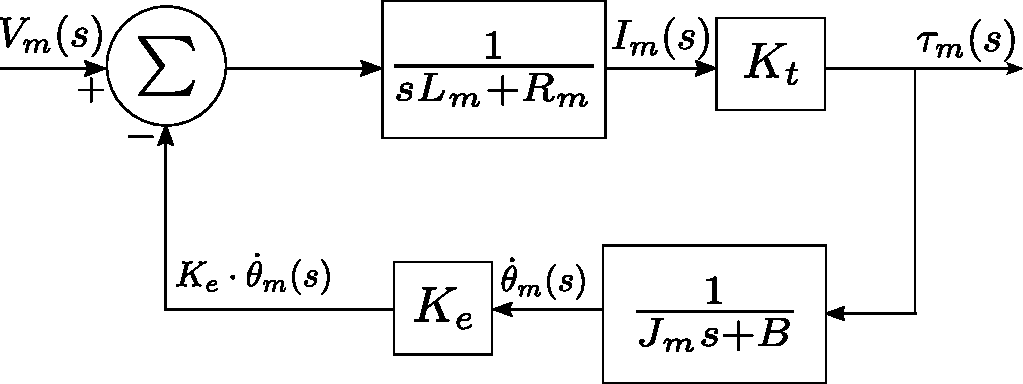
\includegraphics[scale=0.9]{figures/motormodelBlock.pdf}
	\caption{A block representation of the motor, with a voltage, \si{V_m(s)}, as the input and a rotational force, \si{\tau_m(s)}, as the output.}
	\label{fig:motormodelBlock}
\end{figure}

The angular velocity received from the drivetrain, see \figref{fig:Velocitymodelplantopen}, is dependent on the total inertia of the system, and is necessary to ensure the motor is affected by the load.

A model of the electrical and mechanical part has been formed and a block representation of the motor's applied voltage and generated torque has been given. Next step is to model the drivetrain, which connects to the motor through the motor shaft.








It is possible to draw a block diagram for the drivetrain, from the motor torque to the vehicle's velocity with \eqref{eq:TransferFunctionTorqueToVelocity}. Furthermore, the motor needs the produced angular velocity to get affected by the load, i.e. drivetrain. The angular velocity was found in \eqref{eq:BlackBoxGearNewtonLaplaceNew}.

\begin{figure}[H]
	\centering
	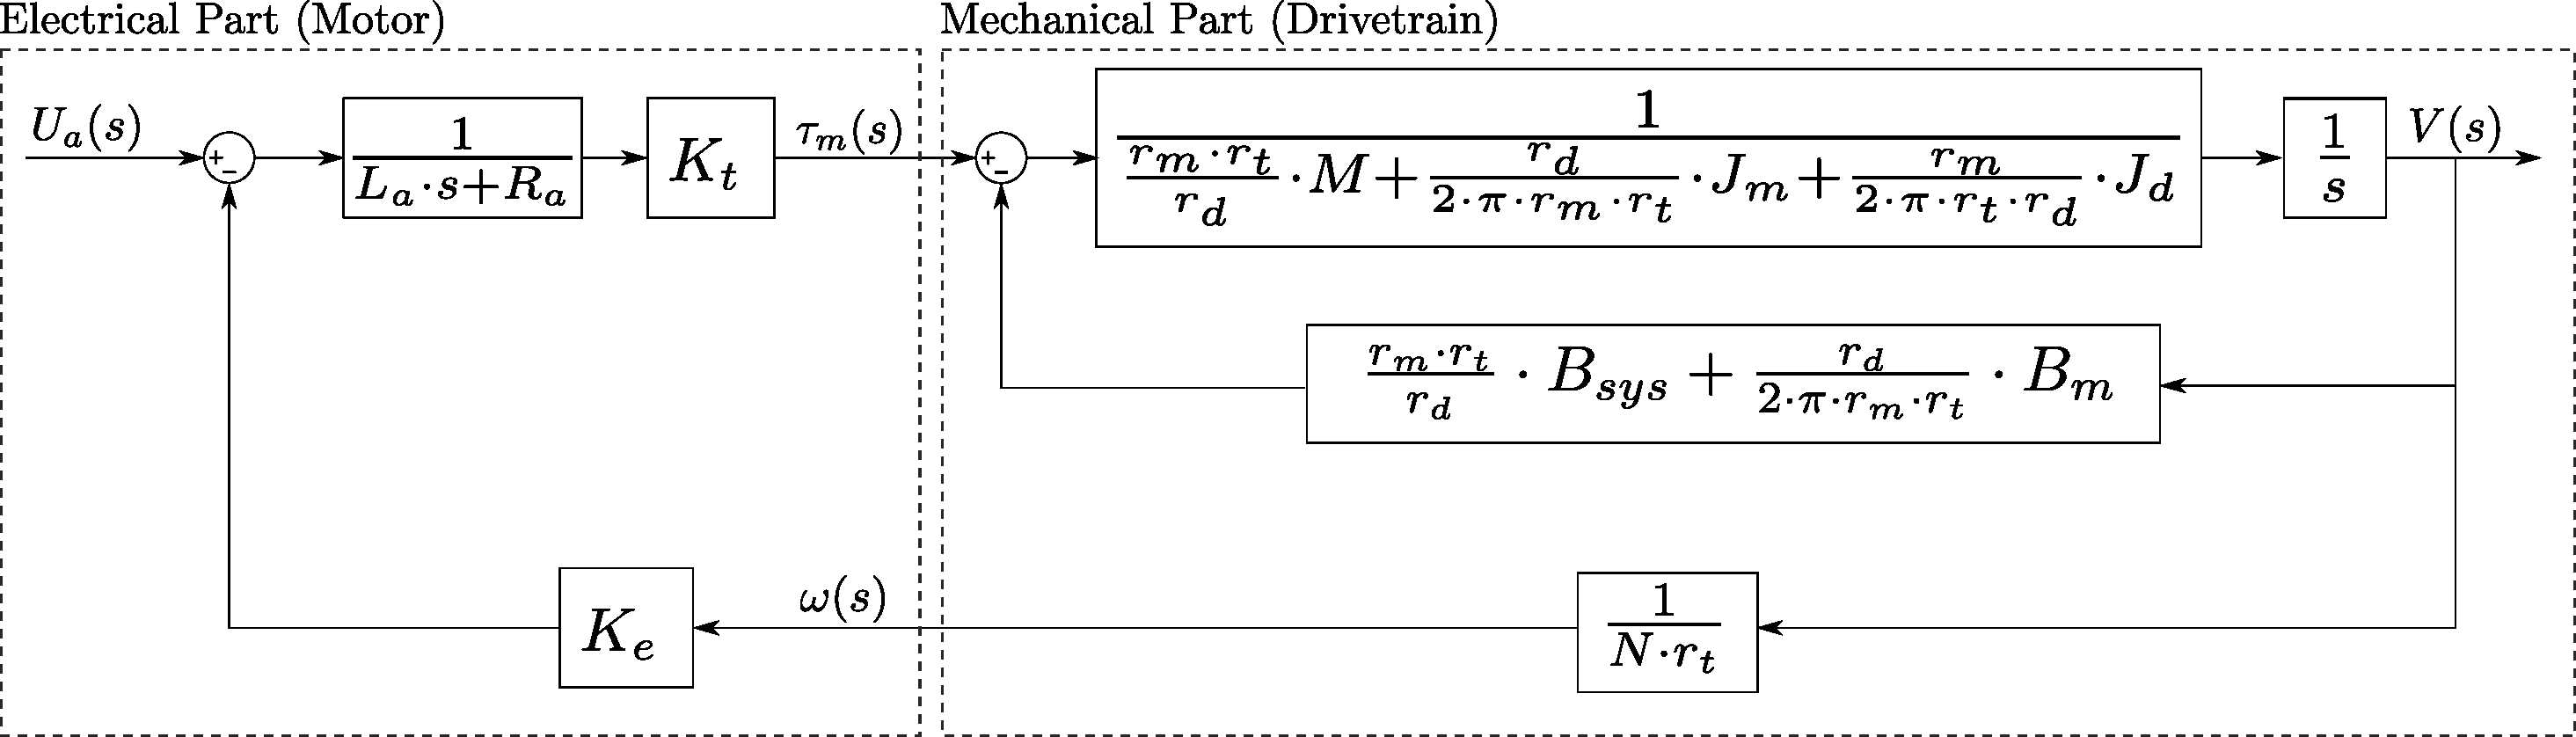
\includegraphics[scale=.28]{figures/totalVelocityModelDiagramComplicated.pdf}
	\caption{A block diagram of the combined drivetrain}
	\label{fig:BlockDiagramDrivetrain}
\end{figure}

%A block diagram describing the drivetrain has been built. In the following section the drivetrain's block diagram is combined with the motor's block diagram, seen in \figref{fig:motormodelBlock}.